%\documentclass[10pt,handout]{beamer}
\documentclass[10pt]{beamer}
\usepackage[english]{babel} % Anpassa efter svenska. Ger svensk logga.
\usepackage[utf8]{inputenc} % Anpassa efter linux
\usepackage{graphicx}
\usepackage{hyperref}
\usepackage{listings}
%\lstdefinelanguage{Stan}{
  morekeywords=[1]{functions,data,parameters,transformed,model,generated,quantities,%
    for,in,while,print,if,else,lower,upper,increment_log_prob,T,return,%
    reject,integrate_ode,integrate_ode_bdf,integrate_ode_rk45,target},%
  morekeywords=[2]{int,real,vector,%
    ordered,positive_ordered,simplex,unit_vector,%
    row_vector,matrix,%
    cholesky_factor_corr,cholesky_factor_cov,%
    coor_matrix,cov_matrix,%
    void},%
  morekeywords=[3]{%
    Phi,%
    Phi_approx,%
    abs,%
    acos,%
    acosh,%
    append_col,%
    append_row,%
    asin,%
    asinh,%
    atan,%
    atan2,%
    atanh,%
    bernoulli_cdf,%
    bernoulli_cdf_log,%
    bernoulli_lccdf,%
    bernoulli_lcdf,%
    bernoulli_logit_lpmf,%
    bernoulli_logit_lpmf,%
    bernoulli_lpmf,%
    bernoulli_lpmf,%
    bernoulli_rng,%
    bessel_first_kind,%
    bessel_second_kind,%
    beta_binomial_cdf,%
    beta_binomial_cdf_log,%
    beta_binomial_lccdf,%
    beta_binomial_lcdf,%
    beta_binomial_lpmf,%
    beta_binomial_lpmf,%
    beta_binomial_rng,%
    beta_cdf,%
    beta_cdf_log,%
    beta_lccdf,%
    beta_lcdf,%
    beta_lpdf,%
    beta_lpdf,%
    beta_rng,%
    binary_log_loss,%
    binomial_cdf,%
    binomial_cdf_log,%
    binomial_coefficient_log,%
    binomial_lccdf,%
    binomial_lcdf,%
    binomial_logit_lpmf,%
    binomial_logit_lpmf,%
    binomial_lpmf,%
    binomial_lpmf,%
    binomial_rng,%
    block,%
    categorical_logit_lpmf,%
    categorical_logit_lpmf,%
    categorical_lpmf,%
    categorical_lpmf,%
    categorical_rng,%
    cauchy_cdf,%
    cauchy_cdf_log,%
    cauchy_lccdf,%
    cauchy_lcdf,%
    cauchy_lpdf,%
    cauchy_lpdf,%
    cauchy_rng,%
    cbrt,%
    ceil,%
    chi_square_cdf,%
    chi_square_cdf_log,%
    chi_square_lccdf,%
    chi_square_lcdf,%
    chi_square_lpdf,%
    chi_square_lpdf,%
    chi_square_rng,%
    cholesky_decompose,%
    col,%
    cols,%
    columns_dot_product,%
    columns_dot_self,%
    cos,%
    cosh,%
    crossprod,%
    csr_extract_u,%
    csr_extract_v,%
    csr_extract_w,%
    csr_matrix_times_vector,%
    csr_to_dense_matrix,%
    cumulative_sum,%
    determinant,%
    diag_matrix,%
    diag_post_multiply,%
    diag_pre_multiply,%
    diagonal,%
    digamma,%
    dims,%
    dirichlet_lpdf,%
    dirichlet_lpdf,%
    dirichlet_rng,%
    distance,%
    dot_product,%
    dot_self,%
    double_exponential_cdf,%
    double_exponential_cdf_log,%
    double_exponential_lccdf,%
    double_exponential_lcdf,%
    double_exponential_lpdf,%
    double_exponential_lpdf,%
    double_exponential_rng,%
    e,%
    eigenvalues_sym,%
    eigenvectors_sym,%
    erf,%
    erfc,%
    exp,%
    exp2,%
    exp_mod_normal_cdf,%
    exp_mod_normal_cdf_log,%
    exp_mod_normal_lccdf,%
    exp_mod_normal_lcdf,%
    exp_mod_normal_lpdf,%
    exp_mod_normal_lpdf,%
    exp_mod_normal_rng,%
    expm1,%
    exponential_cdf,%
    exponential_cdf_log,%
    exponential_lccdf,%
    exponential_lcdf,%
    exponential_lpdf,%
    exponential_lpdf,%
    exponential_rng,%
    fabs,%
    falling_factorial,%
    fdim,%
    floor,%
    fma,%
    fmax,%
    fmin,%
    fmod,%
    frechet_cdf,%
    frechet_cdf_log,%
    frechet_lccdf,%
    frechet_lcdf,%
    frechet_lpdf,%
    frechet_lpdf,%
    frechet_rng,%
    gamma_cdf,%
    gamma_cdf_log,%
    gamma_lccdf,%
    gamma_lcdf,%
    gamma_lpdf,%
    gamma_lpdf,%
    gamma_p,%
    gamma_q,%
    gamma_rng,%
    gaussian_dlm_obs_lpdf,%
    gaussian_dlm_obs_lpdf,%
    get_lp,%
    gumbel_cdf,%
    gumbel_cdf_log,%
    gumbel_lccdf,%
    gumbel_lcdf,%
    gumbel_lpdf,%
    gumbel_lpdf,%
    gumbel_rng,%
    head,%
    hypergeometric_lpmf,%
    hypergeometric_lpmf,%
    hypergeometric_rng,%
    hypot,%
    if_else,%
    inc_beta,%
    int_step,%
    inv,%
    inv_chi_square_cdf,%
    inv_chi_square_cdf_log,%
    inv_chi_square_lccdf,%
    inv_chi_square_lcdf,%
    inv_chi_square_lpdf,%
    inv_chi_square_lpdf,%
    inv_chi_square_rng,%
    inv_cloglog,%
    inv_gamma_cdf,%
    inv_gamma_cdf_log,%
    inv_gamma_lccdf,%
    inv_gamma_lcdf,%
    inv_gamma_lpdf,%
    inv_gamma_lpdf,%
    inv_gamma_rng,%
    inv_logit,%
    inv_phi,%
    inv_sqrt,%
    inv_square,%
    inv_wishart_lpdf,%
    inv_wishart_lpdf,%
    inv_wishart_rng,%
    inverse,%
    inverse_spd,%
    is_inf,%
    is_nan,%
    lbeta,%
    lchoose,%
    lgamma,%
    lkj_corr_cholesky_lpdf,%
    lkj_corr_cholesky_lpdf,%
    lkj_corr_cholesky_rng,%
    lkj_corr_lpdf,%
    lkj_corr_lpdf,%
    lkj_corr_rng,%
    lmgamma,%
    lmultiply,%
    log,%
    log10,%
    log1m,%
    log1m_exp,%
    log1m_inv_logit,%
    log1p,%
    log1p_exp,%
    log2,%
    log_determinant,%
    log_diff_exp,%
    log_falling_factorial,%
    log_inv_logit,%
    log_mix,%
    log_rising_factorial,%
    log_softmax,%
    log_sum_exp,%
    logistic_cdf,%
    logistic_cdf_log,%
    logistic_lccdf,%
    logistic_lcdf,%
    logistic_lpdf,%
    logistic_lpdf,%
    logistic_rng,%
    logit,%
    lognormal_cdf,%
    lognormal_cdf_log,%
    lognormal_lccdf,%
    lognormal_lcdf,%
    lognormal_lpdf,%
    lognormal_lpdf,%
    lognormal_rng,%
    machine_precision,%
    max,%
    mdivide_left_tri_low,%
    mdivide_right_tri_low,%
    mean,%
    min,%
    modified_bessel_first_kind,%
    modified_bessel_second_kind,%
    multi_gp_cholesky_lpdf,%
    multi_gp_cholesky_lpdf,%
    multi_gp_lpdf,%
    multi_gp_lpdf,%
    multi_normal_cholesky_lpdf,%
    multi_normal_cholesky_lpdf,%
    multi_normal_cholesky_rng,%
    multi_normal_lpdf,%
    multi_normal_lpdf,%
    multi_normal_prec_lpdf,%
    multi_normal_prec_lpdf,%
    multi_normal_rng,%
    multi_student_t_lpdf,%
    multi_student_t_lpdf,%
    multi_student_t_rng,%
    multinomial_lpmf,%
    multinomial_lpmf,%
    multinomial_rng,%
    multiply_log,%
    multiply_lower_tri_self_transpose,%
    neg_binomial_2_cdf,%
    neg_binomial_2_cdf_log,%
    neg_binomial_2_lccdf,%
    neg_binomial_2_lcdf,%
    neg_binomial_2_log_lpmf,%
    neg_binomial_2_log_lpmf,%
    neg_binomial_2_log_rng,%
    neg_binomial_2_lpmf,%
    neg_binomial_2_lpmf,%
    neg_binomial_2_rng,%
    neg_binomial_cdf,%
    neg_binomial_cdf_log,%
    neg_binomial_lccdf,%
    neg_binomial_lcdf,%
    neg_binomial_lpmf,%
    neg_binomial_lpmf,%
    neg_binomial_rng,%
    negative_infinity,%
    normal_cdf,%
    normal_cdf_log,%
    normal_lccdf,%
    normal_lcdf,%
    normal_lpdf,%
    normal_lpdf,%
    normal_rng,%
    not_a_number,%
    num_elements,%
    ordered_logistic_lpmf,%
    ordered_logistic_lpmf,%
    ordered_logistic_rng,%
    owens_t,%
    pareto_cdf,%
    pareto_cdf_log,%
    pareto_lccdf,%
    pareto_lcdf,%
    pareto_lpdf,%
    pareto_lpdf,%
    pareto_rng,%
    pareto_type_2_cdf,%
    pareto_type_2_cdf_log,%
    pareto_type_2_lccdf,%
    pareto_type_2_lcdf,%
    pareto_type_2_lpdf,%
    pareto_type_2_lpdf,%
    pareto_type_2_rng,%
    pi,%
    poisson_cdf,%
    poisson_cdf_log,%
    poisson_lccdf,%
    poisson_lcdf,%
    poisson_log_lpmf,%
    poisson_log_lpmf,%
    poisson_log_rng,%
    poisson_lpmf,%
    poisson_lpmf,%
    poisson_rng,%
    positive_infinity,%
    pow,%
    prod,%
    qr_Q,%
    qr_R,%
    quad_form,%
    quad_form_diag,%
    quad_form_sym,%
    rank,%
    rayleigh_cdf,%
    rayleigh_cdf_log,%
    rayleigh_lccdf,%
    rayleigh_lcdf,%
    rayleigh_lpdf,%
    rayleigh_lpdf,%
    rayleigh_rng,%
    rep_array,%
    rep_matrix,%
    rep_row_vector,%
    rep_vector,%
    rising_factorial,%
    round,%
    row,%
    rows,%
    rows_dot_product,%
    rows_dot_self,%
    scaled_inv_chi_square_cdf,%
    scaled_inv_chi_square_cdf_log,%
    scaled_inv_chi_square_lccdf,%
    scaled_inv_chi_square_lcdf,%
    scaled_inv_chi_square_lpdf,%
    scaled_inv_chi_square_lpdf,%
    scaled_inv_chi_square_rng,%
    sd,%
    segment,%
    sin,%
    singular_values,%
    sinh,%
    size,%
    skew_normal_cdf,%
    skew_normal_cdf_log,%
    skew_normal_lccdf,%
    skew_normal_lcdf,%
    skew_normal_lpdf,%
    skew_normal_lpdf,%
    skew_normal_rng,%
    softmax,%
    sort_asc,%
    sort_desc,%
    sort_indices_asc,%
    sort_indices_desc,%
    sqrt,%
    sqrt2,%
    square,%
    squared_distance,%
    step,%
    student_t_cdf,%
    student_t_cdf_log,%
    student_t_lccdf,%
    student_t_lcdf,%
    student_t_lpdf,%
    student_t_lpdf,%
    student_t_rng,%
    sub_col,%
    sub_row,%
    sum,%
    tail,%
    tan,%
    tanh,%
    tcrossprod,%
    tgamma,%
    to_array_1d,%
    to_array_2d,%
    to_matrix,%
    to_row_vector,%
    to_vector,%
    trace,%
    trace_gen_quad_form,%
    trace_quad_form,%
    trigamma,%
    trunc,%
    uniform_cdf,%
    uniform_cdf_log,%
    uniform_lccdf,%
    uniform_lcdf,%
    uniform_lpdf,%
    uniform_lpdf,%
    uniform_rng,%
    variance,%
    von_mises_lpdf,%
    von_mises_lpdf,%
    von_mises_rng,%
    weibull_cdf,%
    weibull_cdf_log,%
    weibull_lccdf,%
    weibull_lcdf,%
    weibull_lpdf,%
    weibull_lpdf,%
    weibull_rng,%
    wiener_lpdf,%
    wiener_lpdf,%
    wishart_lpdf,%
    wishart_lpdf,%
    wishart_rng
  },%
  otherkeywords={<-,~,+=,=},%
  sensitive=true,%
  morecomment=[l]{\#},%
  morecomment=[l]{//},%
  morecomment=[n]{/*}{*/},%
  string=[d]"%,
  literate={<-}{{$\leftarrow$}}1 {~}{{$\sim$}}1%
}
 % Stan listing
\usepackage{lstbayes}
\usepackage[all,poly,ps,color]{xy}


\hypersetup{
    colorlinks=true,
    linkcolor=blue,
    filecolor=magenta,
    urlcolor=cyan,
}
\usepackage{../common/beamerthemeUppsala}
%\usetheme{Uppsala}
%\usecolortheme{UU} % Anpassa efter UU:s frger och logga
%\hypersetup{pdfpagemode=FullScreen} % Adobe Reader ska ppna fullskrm
\setbeamertemplate{itemize items}[circle]

% \usepackage{beamerthemesplit}
\usepackage{amsmath,amsfonts,amssymb}
% \usepackage{amssymb}
% \usepackage{graphics}
% \usepackage{graphicx}
% \usepackage{epsfig}
% \usepackage[latin1]{inputenc}
 \usepackage{color}
% \usepackage{fancybox}
% \usepackage{psfrag}
% \usepackage[english]{babel}
 \setbeamertemplate{footline}{\hfill\insertframenumber/\inserttotalframenumber}

% Input new commands
%\usepackage{bm}
%\usepackage{natbib}
\newcommand{\bfm}[1]   {\mbox{\boldmath{${#1}$}}}
\newcommand{\Prob}   {\mbox{\textnormal{P}}}
\def\eqd{\,{\buildrel d \over =}\,}

% Vector/Matrix definitions (in bold type)
\newcommand{\vect}[1]{\mathbf{#1}}
\newcommand{\vectb}[1]{\bm{#1}}

% Differential operator 'd' as upright as in (use \dd)
\newcommand{\dd}{\; \mathrm{d}}

% Gaussian normal distribution (use \N)
\newcommand{\N}{\mathcal{N}} %% or \mathrm{N}

% Uniform distribution (use \Uni or \U)
\newcommand{\Uni}{\mathcal{U}} %% or \mathrm{U}
\newcommand{\U}{\mathcal{U}} %% or \mathrm{U}

% Matrix transpose (use \T)
\newcommand{\T}{^{\mathsf{T}}}

% Blockdiagonal matrices (use \blockdiag)
\newcommand{\blockdiag}{\mathrm{blockdiag}}

% Define inner product '<f,g>' notation (use \innerp{#1})
\providecommand{\innerp}[1]{\left\langle#1\right\rangle}

\def\o{{\mathbf o}}
\def\t{{\mathbf \theta}}
\def\w{{\mathbf w}}
\def\x{{\mathbf x}}
\def\y{{\mathbf y}}
\def\z{{\mathbf z}}



% Other math symbols and notation
\newcommand{\D}{^\mathsf{\dagger}}
\newcommand{\R}{\mathbb{R}}
\newcommand{\erf}{\mathrm{erf}}
\newcommand{\E}{\mathrm{E}}
\newcommand{\var}{\mathrm{var}}
\newcommand{\Var}{\mathrm{Var}}
\newcommand{\cov}{\mathrm{cov}}
\newcommand{\Ker}{\operatorname{Ker}}
\newcommand{\Ran}{\operatorname{Ran}}
\providecommand{\norm}[1]{\lVert#1\rVert}
\providecommand{\op}[1]{\mathcal{#1}}
\newcommand{\arccot}{\mathrm{arccot}}
\providecommand{\Hspace}[1]{\mathscr{#1}}
\providecommand{\fourier}[1]{\mathscr{#1}}

\newcommand{\kin}{k^{\rm in}}
\newcommand{\kout}{k^{\rm out}}
\newcommand{\gi}{{R_0}}
\newcommand{\eff}{{E_{\rm max}}}
\newcommand{\ESS}{\mathrm{ESS}}
\newcommand{\HN}{{\rm N^+}}
\newcommand{\lN}{{\rm LN}}

\DeclareMathOperator{\Sd}{Sd}
\DeclareMathOperator{\sd}{sd}
\DeclareMathOperator{\Gammad}{Gamma}
\DeclareMathOperator{\Invgamma}{Inv-gamma}
\DeclareMathOperator{\Bin}{Bin}
\DeclareMathOperator{\Negbin}{Neg-bin}
\DeclareMathOperator{\Poisson}{Poisson}
\DeclareMathOperator{\Beta}{Beta}
\DeclareMathOperator{\logit}{logit}
\DeclareMathOperator{\BF}{BF}
\DeclareMathOperator{\Invchi2}{Inv-\chi^2}
\DeclareMathOperator{\NInvchi2}{N-Inv-\chi^2}
\DeclareMathOperator{\InvWishart}{Inv-Wishart}
\DeclareMathOperator{\tr}{tr}
% \DeclareMathOperator{\Pr}{Pr}
\def\euro{{\footnotesize \EUR\, }}
\DeclareMathOperator{\rep}{\mathrm{rep}}


\def\dashxy(#1){%
  /xydash{[#1] 0 setdash}def}
\def\grayxy(#1){%
  /xycolor{#1 setgray}def}
\newgraphescape{D}[1]{!{\ar @*{[!\dashxy(2 2)]} "#1"}}
\newgraphescape{P}[1]{!{\ar "#1"}}
\newgraphescape{F}[1]{!{*+=<2em>[F=]{#1}="#1"}}
\newgraphescape{O}[1]{!{*+=<2em>[F]{#1}="#1"}}
\newgraphescape{V}[1]{!{*+=<2em>[o][F]{#1}="#1"}}
\newgraphescape{B}[3]{!{{ "#1"*+#3\frm{} }.{ "#2"*+#3\frm{} } *+[F:!\grayxy(0.75)]\frm{}}}

%%%%%%%%%%%%%%%%%%%%%%%%%%%%%%%%%%%%%%%%%%%%%%%%%%%%%%%%%%%%%%%%%%

\setlength{\parskip}{3mm}
\title[]{{\color{black}Bayesian Statistics and Data Analysis \\ Lecture 7}}
\author[]{M{\aa}ns Magnusson \\ Department of Statistics, Uppsala University \\ Thanks to Aki Vehtari, Aalto University}
\date{}

\begin{document}

\frame{\titlepage
% \thispagestyle{empty}
}

%%%%%%%%%%%%%%%%%%%%%%%%%%%%%%%%%%%%%%%%%%%%%%%%%%%%%%%%%%%%%%%%%%


\section{Hierarchical models}
\frame{\sectionpage}

\begin{frame}

\frametitle{Hierarchical model}

  \begin{itemize}
  \item Example: Treatment effectiveness
    \begin{itemize}
    \item in hospital $j$ the survival probability is $\theta_j$
    \item observations $y_{ij}$ tell whether patient $i$ survived in
      hospital $j$
        \begin{xy}
          \xymatrix{ \theta_1\ar[d] & \theta_2\ar[d] &
            \cdots & \theta_n\ar[d] \\
            y_{i1} & y_{i2} & & y_{in} }
        \end{xy}
        \pause
      \item sensible to assume that $\theta_j$ are similar
        \begin{xy}
          \xymatrix{
            & \tau \ar[dl] \ar[d] \ar[drr] & & &  \\
            \theta_1\ar[d] & \theta_2\ar[d] &
            \cdots & \theta_n\ar[d] \\
            y_{i1} & y_{i2} & & y_{in} }
        \end{xy}
%        \pause
      \item natural to think that $\theta_j$ have common population distribution
      \item $\theta_j$ is not directly observed and the population distribution is unknown
    \end{itemize}
  \end{itemize}
\end{frame}

\begin{frame}[fragile]

\frametitle{Hierarchical model: terms}

\begin{overlayarea}{8cm}{4cm}
  \begin{itemize}
  \item[Lvl 1:] observations given parameters $p(y_{ij}|\theta_j)$
  \item<2->[Lvl 2:] parameters given hyperparameters
    $p(\theta_j|\tau)$
  \end{itemize}
  \begin{minipage}[b]{3cm}
  \scriptsize
    \begin{xy}
      \xymatrix{
        p(\tau) & & \tau \ar[dl] \ar[d] \ar[drr] & & & \text{hyperparameter} \\
        p(\theta_j|\tau) & \theta_1\ar[d] & \theta_2\ar[d] & \cdots &
        \theta_n\ar[d] & \text{parameters} \\
        p(y_{ij}|\theta_j) & y_{i1} & y_{i2} &  & y_{in} & \text{observations}
      }
    \end{xy}
  \end{minipage}\\
%  \only<1>{\hide[white]{-0.3}{-0.2}{0.13}{1.2}} %
\end{overlayarea}
\vspace{1cm}
  Joint posterior
  \begin{eqnarray*}
    p(\theta,\tau|y) & \propto & p(y|\theta,\tau) p(\theta,\tau) \\
    & \propto & p(y|\theta) p(\theta|\tau) p(\tau)
  \end{eqnarray*}
\end{frame}

\begin{frame}

\frametitle{Comparisons}
	\begin{itemize}
    \item<+-> "Separate model" (model with separate/independent effects)
        \begin{xy}
          \xymatrix{ \theta_1\ar[d] & \theta_2\ar[d] &
            \cdots & \theta_n\ar[d] \\
            y_{1} & y_{2} & & y_{n} }
        \end{xy}
     \item<+-> "Joint/pooled model" (model with a common effect / pooled model)
        \begin{xy}
          \xymatrix{
            & \theta \ar[dl] \ar[d] \ar[drr] & & &  \\
            y_{1} & y_{2} & \cdots & y_{n}}        \end{xy}
      \item<+-> Hierarchical model\\
        \vspace{-.5\baselineskip}\hspace{0cm}
        \begin{xy}
          \xymatrix{
            & \tau \ar[dl] \ar[d] \ar[drr] & & &  \\
            \theta_1\ar[d] & \theta_2\ar[d] &
            \cdots & \theta_n\ar[d] \\
            y_{1} & y_{2} & & y_{n} }
        \end{xy}
  \end{itemize}

\end{frame}

\begin{frame}
\frametitle{Predictive distributions for hiearchical models}

  \begin{itemize}
    \item Two types of predictive distributions
    \begin{enumerate}
      \item A new observation in {\color{uured} an existing group}
      \item A new observation in {\color{uured} a new group}
    \end{enumerate}
        \begin{xy}
          \xymatrix{
            & \tau \ar[dl] \ar[d] \ar[drr] & & &  \\
            \theta_1\ar[d] & \theta_2\ar[d] &
            \cdots & \theta_n\ar[d] \\
            y_{1} & y_{2} & & y_{n} }
        \end{xy}
  \end{itemize}
\end{frame}

\subsection{Rats example}

\begin{frame}

\frametitle{Hierarchical binomial model: rats}

  \begin{itemize}
  \item Medicine testing
  \item Type F344 female rats in control group given placebo
    \begin{itemize}
    \item count how many get endometrial stromal polyps
    \item familiar binomial model example
    \end{itemize}
  \item<2-> Experiment has been repeated 71 times
    {\tiny
      \begin{tabular}{r r r r r r r r r r}
        0/20 & 0/20 & 0/20 & 0/20 & 0/20 & 0/20 & 0/20 & 0/19 & 0/19 & 0/19 \\
        0/19 & 0/18 & 0/18 & 0/17 & 1/20 & 1/20 & 1/20 & 1/20 & 1/19 & 1/19 \\
        1/18 & 1/18 & 2/25 & 2/24 & 2/23 & 2/20 & 2/20 & 2/20 & 2/20 & 2/20 \\
        2/20 & 1/10 & 5/49 & 2/19 & 5/46 & 3/27 & 2/17 & 7/49 & 7/47 & 3/20 \\
        3/20 & 2/13 & 9/48 & 10/50 & 4/20 & 4/20 & 4/20 & 4/20 & 4/20 & 4/20 \\
        4/20 & 10/48 & 4/19 & 4/19 & 4/19 & 5/22 & 11/46 & 12/49 & 5/20 & 5/20 \\
        6/23 & 5/19 & 6/22 & 6/20 & 6/20 & 6/20 & 16/52 & 15/46 & 15/47 & 9/24 \\
        4/14 &      &      &      &      &      &       &       &       &
      \end{tabular}}
  \end{itemize}

\end{frame}

\begin{frame}

\frametitle{Hierarchical binomial model: rats}

  \only<1>{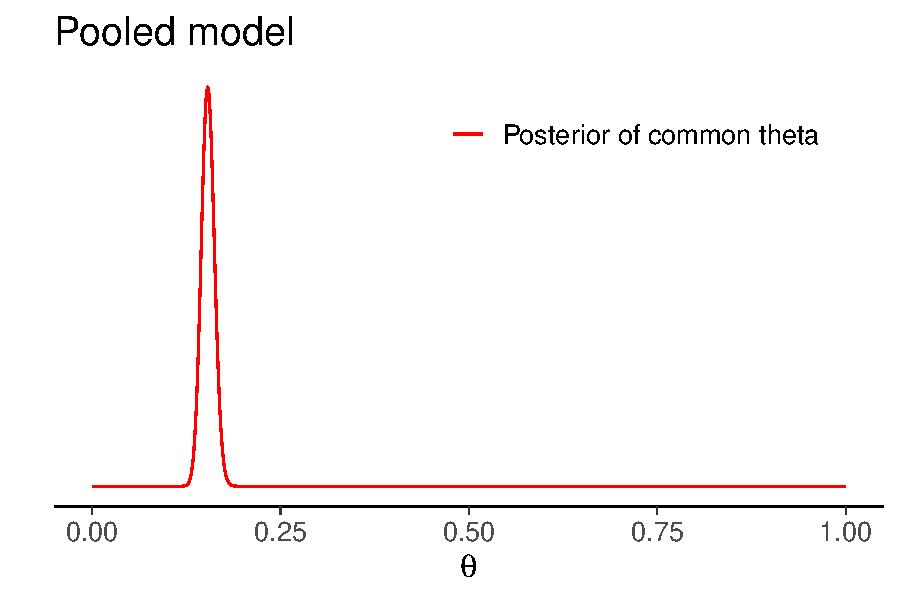
\includegraphics[width=9cm]{figs/rats_pooled.pdf}}
  \only<2>{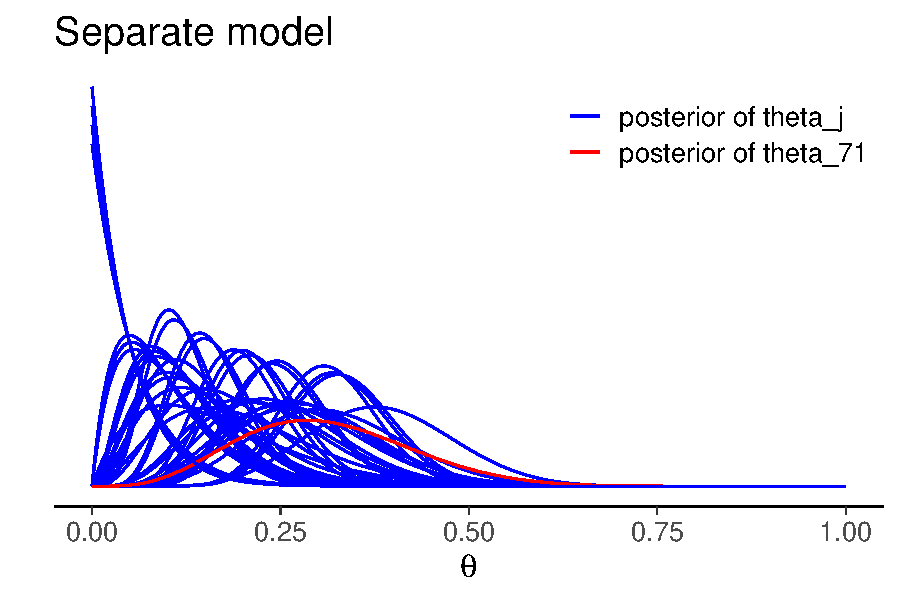
\includegraphics[width=9cm]{figs/rats_separate.pdf}}


\end{frame}

\begin{frame}[fragile]

\frametitle{Hierarchical binomial model: rats}

  \begin{itemize}
  \item Hierarchical binomial model for rats\\
    prior parameters {\color{red} $\alpha$} and {\color{red} $\beta$} are unknown
\end{itemize}
    \begin{minipage}[t]{4cm}
      \xygraph{
        []              !O{y_j}
        ([u]   !V{{\color{uulgr}\theta_j}}  !P{y_j}
        ([u][l(0.33)] !V{\color{red} \alpha} !P{{\color{uulgr}\theta_j}},
        [u][r(0.33)] !V{\color{red} \beta}  !P{{\color{uulgr}\theta_j}}),
        [u][r(0.75)]  !F{n_j}    !P{y_j},
        [r(1.0)]*{j},
        [l(3.0)]*{y_j|n_j,{\color{uulgr}\theta_j} \sim \Bin(y_j|n_j,{\color{uulgr}\theta_j})},
        [u][l(2.93)]*{{\color{uulgr}\theta_j}|{\color{red}\alpha,\beta} \sim
          \Beta({\color{uulgr}\theta_j}|{\color{red}\alpha,\beta})},
        [l(6.0)]*{~}
        )
        !B{{\color{uulgr}\theta_j}}{j}{++}
      }
    \end{minipage}
    %\pause
  \begin{itemize}
    \item Joint posterior
      $p({\color{uulgr}\theta_1,\ldots,\theta_J},{\color{red}\alpha},{\color{red}\beta}|y)$
      \begin{itemize}
    \item multiple parameters
      \pause
      \item factorize
        $\prod_{j=1}^J p({\color{uulgr}\theta_j}|{\color{red}\alpha,\beta},y)p({\color{red}\alpha,\beta}|y)$
\end{itemize}
\end{itemize}
\end{frame}

\begin{frame}

\frametitle{Hierarchical binomial model: rats}

  \begin{itemize}
  \item Population prior $\Beta({\color{uulgr}\theta_j}|{\color{red}\alpha,\beta})$
  \item Hyperprior $p({\color{red}\alpha,\beta})$?
    \begin{itemize}
    \item ${\color{red}\alpha,\beta}$ both affect the location and scale
    \item BDA3 (p. 110) has (vague)
      $p({\color{red}\alpha,\beta})\propto({\color{red}\alpha}+{\color{red}\beta})^{-5/2}$
    \end{itemize}
    \pause
    \item {\color{uured} What type of predicitive distributions can we have?}
    \end{itemize}
\end{frame}

\begin{frame}

\frametitle{Hierarchical binomial model: rats}

  \only<1>{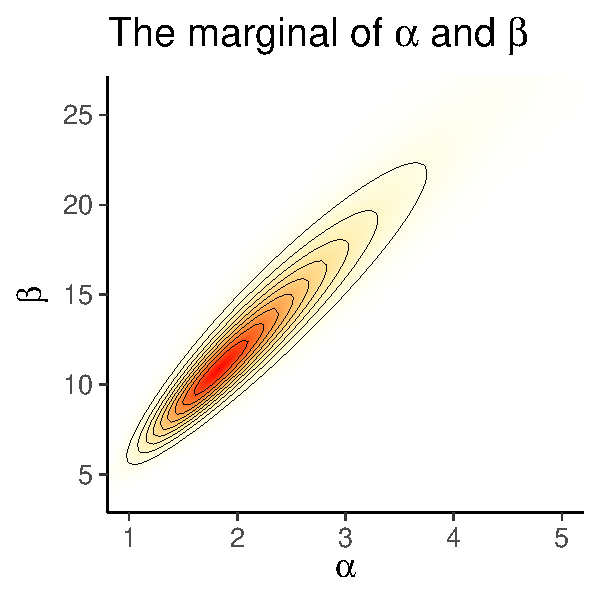
\includegraphics[width=8cm]{figs/rats_posterior.pdf}}
  \only<2>{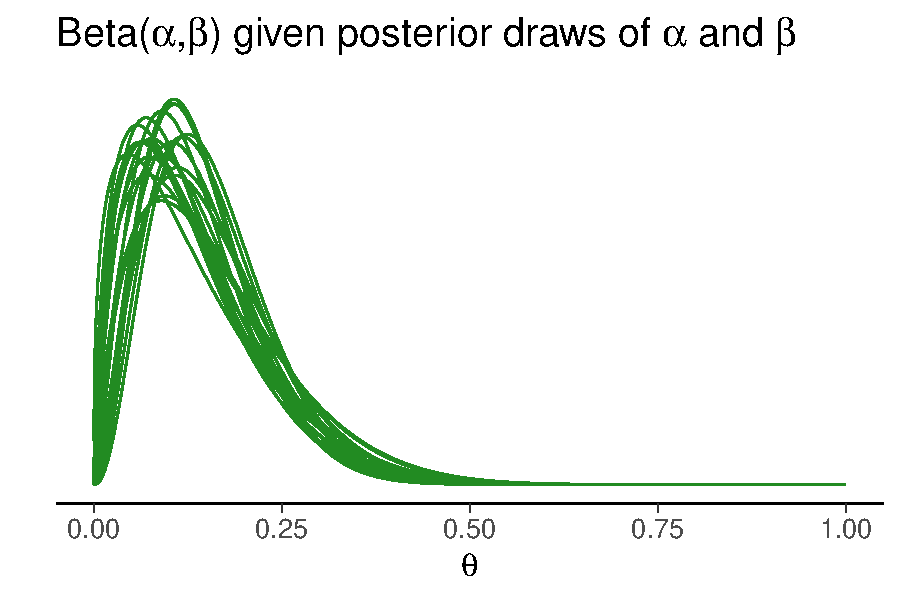
\includegraphics[width=8cm]{figs/rats_hierdraws.pdf}}
  \only<3>{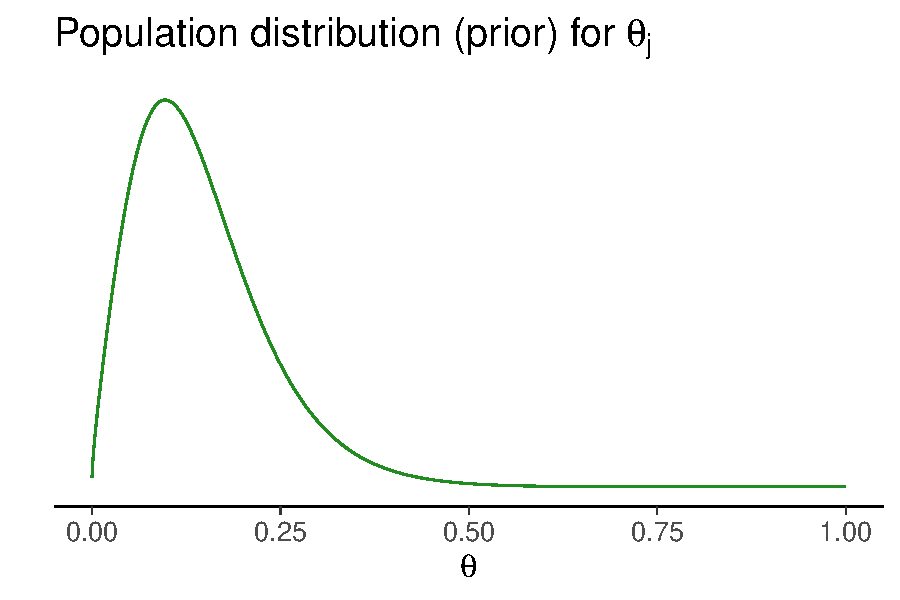
\includegraphics[width=8cm]{figs/rats_hierprior.pdf}}
  \only<4-5>{\vspace{-0.3\baselineskip}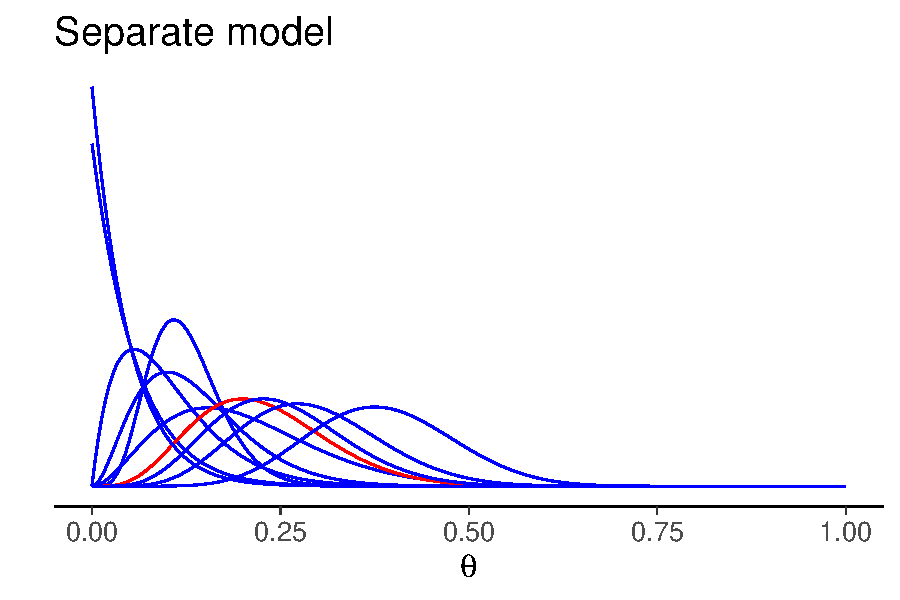
\includegraphics[width=6.7cm]{figs/rats_separate_less.pdf}\\}
  \only<5-6>{\vspace{-0.3\baselineskip}
    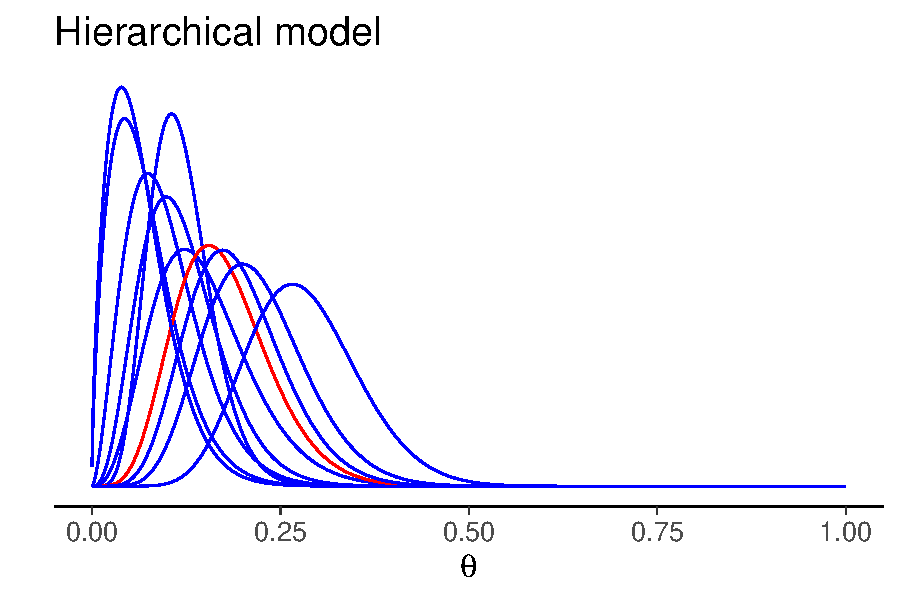
\includegraphics[width=6.7cm]{figs/rats_hier_less.pdf}\\}
  \only<6>{\vspace{-0.3\baselineskip}
    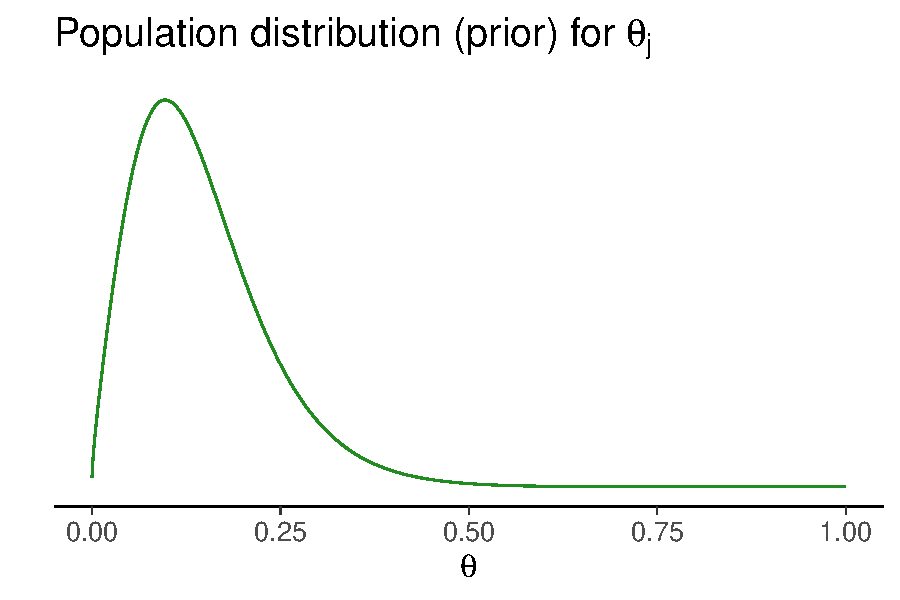
\includegraphics[width=6.7cm]{figs/rats_hierprior.pdf}\\}


\end{frame}

\subsection{Factory example}

\begin{frame}

\frametitle{Hierarchical normal model: factory}

  \begin{itemize}
  \item Factory has 6 machines which quality is evaluated
  \item Assume hierarchical model
    \begin{itemize}
    \item each machine has its own (average) quality $\theta_j$ and
      {\color{uured} common variance} $\sigma^2$
    \end{itemize}
\begin{minipage}[b]{4cm}
\begin{xy}
\xygraph{
  []              !O{y_{ij}}
 ([u][l(0.75)]   !V{\theta_j}      !P{y_{ij}}
 ([u][l(0.33)] !V{\mu_P}      !P{\theta_j},
   [u][r(0.33)] !V{\sigma_P^2} !P{\theta_j}),
  [u][r(1.75)]   !V{\sigma^2}   !P{y_{ij}},
  [r(0.45)]*{i},
  [r(0.9)]*{j},
[l(3)]*{y_{ij}|\theta_j \sim \N(\theta_j,\sigma^2)},
[u][l(3)]*{\theta_j|\mu_P,\sigma_P^2 \sim \N(\mu_P,\sigma_P^2)},
)
!B{y_{ij}}{i}{}
!B{\theta_j}{j}{++}
 }
\end{xy}
    \end{minipage}
  \item Can be used to predict the future quality produced by each machine and quality produced by a new similar machine
  \end{itemize}
\end{frame}

\begin{frame}

\frametitle{Hierarchical normal model: factory}

  \begin{itemize}
  \item Factory has 6 machines which quality is evaluated
  \item Assume hierarchical model
    \begin{itemize}
    \item each machine has its own (average) quality $\theta_j$ and
      {\color{uured} own variance} $\sigma_j^2$
    \end{itemize}
\hspace{-1cm}~\begin{minipage}[b]{4cm}
      \begin{xy}
        \xygraph{
          []              !O{y_{ij}}
          ([u][l(0.75)]   !V{\theta_j}      !P{y_{ij}}
          ([u][l(0.33)] !V{\mu_P}      !P{\theta_j},
          [u][r(0.33)] !V{\sigma_P^2} !P{\theta_j}),
          [u][r(0.75)]   !V{\sigma_j^2}   !P{y_{ij}}
          ([u][l(0.33)] !V{\sigma_0^2}      !P{\sigma_j^2},
          [u][r(0.33)] !V{\nu_0} !P{\sigma_j^2}),
          [r(0.45)]*{i},
          [r(0.9)]*{j},
          [l(3.0)]*{y_{ij}|\theta_j \sim \N(\theta_j,\sigma_j^2)},
          [u][l(3.0)]*{\theta_j|\mu_P,\sigma_P^2 \sim \N(\mu_P,\sigma_P^2)},
          [u][r(3.25)]*{\sigma_j^2|\sigma_0^2,\nu_0 \sim \Invchi2(\sigma_0^2,\nu_0)}
          )
          !B{y_{ij}}{i}{}
          !B{\theta_j}{j}{++}
        }
      \end{xy}
    \end{minipage}
    \pause
  \item {\color{uured} What type of predicitive distributions can we have?}
    \pause
  \item Can be used to predict the future quality produced by each machine and quality produced by a new similar machine
  \end{itemize}
\end{frame}

\subsection{8 schools example}

\begin{frame}

\frametitle{Hierarchical normal model: 8 schools}

  \begin{itemize}
  \item Example: SAT coaching effectiveness
    \begin{itemize}
    \item in USA commonly used Scholastic Aptitude Test (SAT) is
      designed so that short term practice should not improve the
      results significantly
    \item schools have anyway coaching courses
    \item test the effectiveness of the coaching courses
    \end{itemize}
    \pause
  \item SAT
    \begin{itemize}
    \item standardized multiple choice test
    \item mean about 500 and standard deviation about 100
    \item most scores between 200 and 800
    \item different topics, e.g., V=Verbal, M=Mathematics
    \item pre-test PSAT
    \end{itemize}
\end{itemize}
\end{frame}

\begin{frame}

\frametitle{Hierarchical normal model: 8 schools}

  \begin{itemize}
  \item Effectiveness of the SAT coaching
    \begin{itemize}
    \item students had made pre-tests PSAT-M and
      PSAT-V
    \item part of students were coached
    \item linear regression was used to estimate the coaching effect
      $y_j$ for the school $j$ (could be denoted with $\bar{y}_{.j}$,
      too) and variances $\sigma_j^2$
    \item $y_j$ approximately normally distributed, with variances
      assumed to be known based on about 30 students per school
    \item data is group means and variances (not personal results)
    \end{itemize}
    \pause
  \item Data:
    {\small
    \begin{tabular}[t]{r | r r r r r r r r}
      School & A & B & C & D & E & F & G & H \\
      $y_j$ & 28 & 8 & -3 & 7 & -1 & 1 & 18 & 12 \\
      $\sigma_j$ & 15 & 10 & 16 & 11 & 9 & 22 & 20 & 28
    \end{tabular}}
  \end{itemize}
\end{frame}

\begin{frame}

\frametitle{Hierarchical normal model for group means}

  \begin{itemize}
  \item $J$ experiments, unknown $\theta_j$ and known $\sigma^2$
    \begin{equation*}
      y_{ij}|\theta_j \sim \N(\theta_j,\sigma^2), \quad
      i=1,\ldots,n_j; \quad j=1,\ldots,J
    \end{equation*}
    \vspace{-6mm}
  \item Group $j$ sample mean and sample variance
    \begin{eqnarray*}
      \bar{y}_{.j} & = & \frac{1}{n_j}\sum_{i=1}^{n_j}y_{ij}\\
      \sigma_j^2 & = & \frac{\sigma^2}{n_j}
    \end{eqnarray*}
    \vspace{-6mm}
    \pause
  \item Use model
    \begin{eqnarray*}
      \bar{y}_{.j}|\theta_j \sim \N(\theta_j,\sigma_j^2)
    \end{eqnarray*}
     this model can be generalized so that, $\sigma_j^2$ can be
    different from each other for other reasons than $n_j$
  \end{itemize}
\end{frame}

\begin{frame}

\frametitle{Hierarchical normal model for group means}

    \begin{minipage}[b]{4cm}
      \begin{xy}
        \xygraph{
          []              !O{\bar{y}_{.j}}
          ([u][l(0.5)]   !V{\theta_j}      !P{\bar{y}_{.j}}
          ([u][l(0.33)] !V{\mu}      !P{\theta_j},
          [u][r(0.33)] !V{\tau} !P{\theta_j}),
          [u][r(0.5)]   !O{\sigma_j^2}   !P{\bar{y}_{.j}},
  [r(1.0)]*{j},
  [l(3.0)]*{\bar{y}_{.j}|\theta_j \sim \N(\theta_j,\sigma^2_j)},
  [u][l(3.0)]*{\theta_j|\mu,\tau \sim \N(\mu,\tau)}
  )
  !B{\theta_j}{j}{++}
}
\end{xy}
\end{minipage}
\end{frame}

\begin{frame}

\frametitle{Hierarchical normal model: 8 schools}

  \only<1-3>{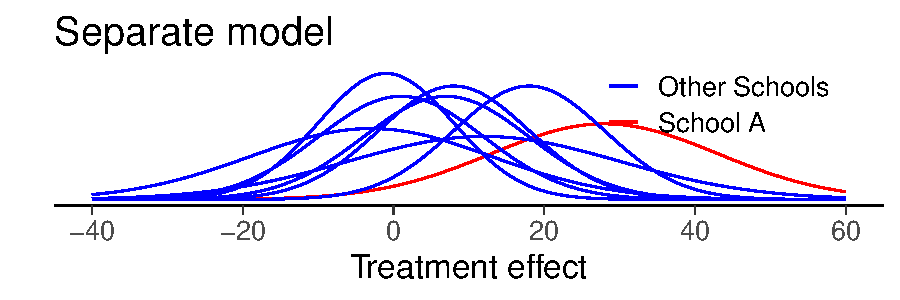
\includegraphics[width=8.3cm]{figs/8schools_separate.pdf}\\}
  \only<2-3>{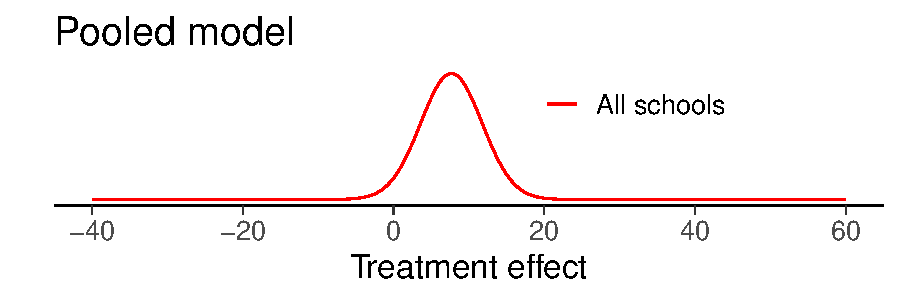
\includegraphics[width=8.3cm]{figs/8schools_pooled.pdf}\\}
  \only<3>{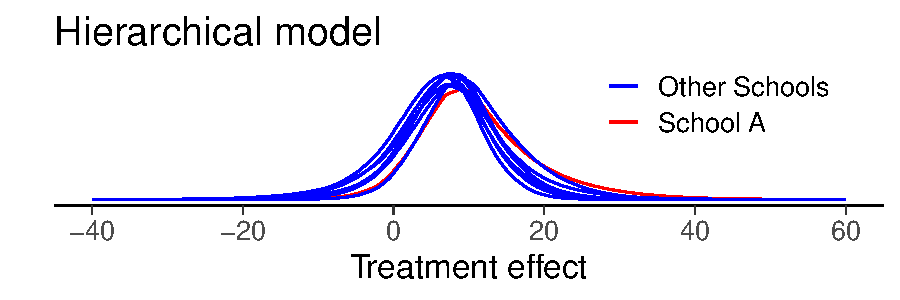
\includegraphics[width=8.3cm]{figs/8schools_hier.pdf}}
  \only<4-6>{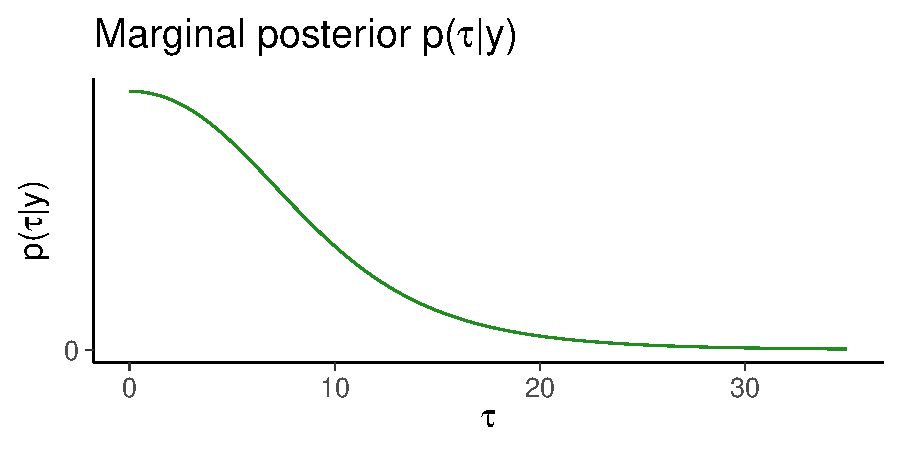
\includegraphics[width=5.5cm]{figs/8schools_tau.pdf}\\}
  \only<5-6>{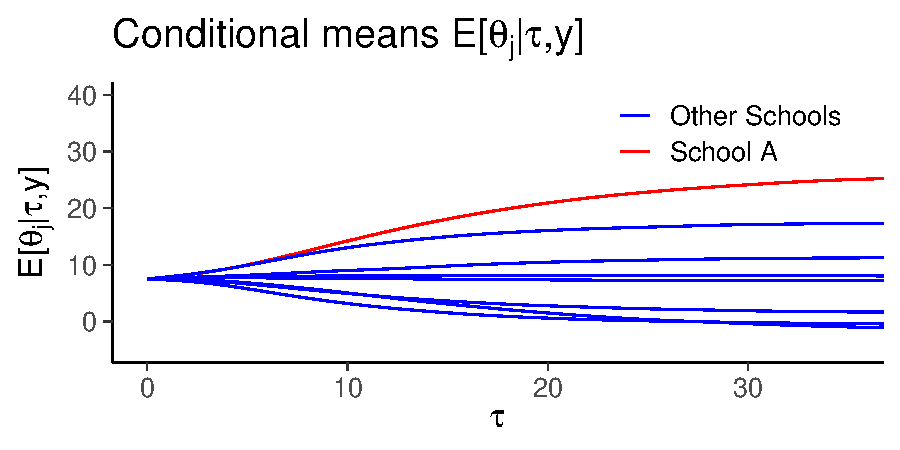
\includegraphics[width=5.5cm]{figs/8schools_condmu.pdf}\\}
  \only<6>{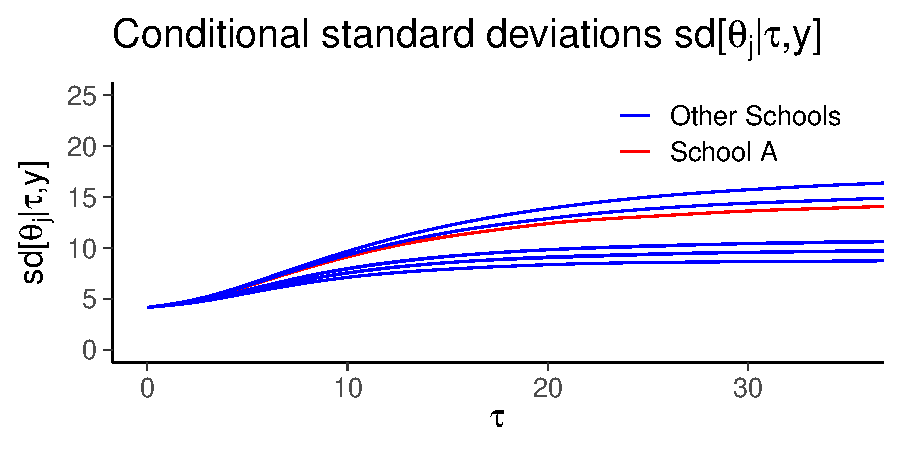
\includegraphics[width=5.5cm]{figs/8schools_condsd.pdf}}

\end{frame}


\section{Exchangeability}
\frame{\sectionpage}

\begin{frame}

\frametitle{Exchangeability}

  \begin{itemize}
  \item Justifies why we can use
    \begin{itemize}
    \item a joint model for data
    \item a joint prior for a set of parameters
    \end{itemize}
  \item Less strict than independence (IID)
  \item IID $\rightarrow$ exchangeability
  \end{itemize}
\end{frame}

\begin{frame}

\frametitle{Exchangeability}

  \begin{itemize}
  \item \textit{Exchangeability} \\ Parameters
    $\theta_1,\ldots,\theta_J$ (or observations $y_1,\ldots,y_J$) are
    exchangeable if the joint distribution $p$ is invariant to the
    permutation of indices $(1,\ldots,J)$\\
  e.g.
    \begin{equation*}
      p(\theta_1,\theta_2,\theta_3) = p(\theta_2,\theta_3,\theta_1)
    \end{equation*}

  \item Exchangeability implies symmetry: \\If there is no information
    which can be used \textit{a priori} to separate $\theta_j$ form
    each other, we can assume exchangeability. ("Ignorance implies exchangeability")

  \end{itemize}
\end{frame}


\begin{frame}

\frametitle{Exchangeability}

  \begin{itemize}
  \item Exchangeability does not mean that the results of the
    experiments could not be different
    \begin{itemize}
    \item e.g. if we know that the experiments have been in two
      different laboratories, and we know that the other laboratory
      has better conditions for the rats, but we do not know which
      experiments have been made in which laboratory
    \item a priori experiments are exchangeable
    \item model could have unknown parameter for the laboratory with a
      conditional prior for rats assumed to come form the same place (clustering model)
    \end{itemize}
  \end{itemize}
\end{frame}

% \note{Elinolojen parantaminen vaikutti
\begin{frame}

\frametitle{Exchangeability and additional information}

  \begin{itemize}
  \item Example: bioassay
    \begin{itemize}
      \item<+-> $y_i$ number of dead animals are not exchangeable alone
      \item<+-> $x_i$ dose is additional information
      \item<+-> $(x_i,y_i$) exchangeable and logistic regression was used
    \begin{align*}
      p(\alpha,\beta|y,n,x)\propto \prod_{i=1}^n p(y_i|\alpha,\beta,n_i,x_i)p(\alpha,\beta)
    \end{align*}
    \end{itemize}
  \end{itemize}
\end{frame}

\begin{frame}

\frametitle{Hierarchical exchangeability}

  \begin{itemize}
  \item Example: hierarchical rats example
    \begin{itemize}
    \item<+-> all rats not exchangeable
    \item<+-> in a single laboratory rats exchangeable
    \item<+-> laboratories exchangeable
    \item<+-> $\rightarrow$ hierarchical model can be used
    \end{itemize}
  \end{itemize}
\end{frame}

\begin{frame}

\frametitle{Partial or conditional exchangeability}

\begin{itemize}
  \item Conditional exchangeability
    \begin{itemize}
    \item if $y_i$ is connected to an additional information $x_i$, so
      that $y_i$ are not exchangeable, but $(y_i,x_i)$ exchangeable
      use joint model or conditional model $(y_i|x_i)$.
    \end{itemize}
  \item<2-> Partial exchangeability
    \begin{itemize}
    \item if the observations can be grouped (a priori), then use
      hierarchical model
    \end{itemize}
\end{itemize}
\end{frame}

\begin{frame}

\frametitle{Exchangeability}

  \begin{itemize}
  \item The simplest form of the exchangeability (but not the only
    one) for the parameters $\theta$ conditional independence
    \begin{equation*}
      p(x_1,\ldots,x_J|\theta)=\prod_{j=1}^J p(x_j|\theta)
    \end{equation*}
  \item<2-> Let $(x_n)_{n=1}^{\infty}$ to be an infinite sequence of
    exchangeable random variables. De Finetti's theorem then says that
    there is some random variable $\theta$ so that $x_j$ are
    conditionally independent given $\theta$, and joint density for
    $x_1,\ldots,x_J$ can be written in the \textit{iid mixture} form
    \begin{equation*}
      p(x_1,\ldots,x_J)=\int \left[\prod_{j=1}^J p(x_j|\theta)\right]p(\theta)d\theta
    \end{equation*}

  %   \vspace{-6mm}
  % \item marginal distribution of $\theta$
  %   \begin{equation*}
  %     p(\theta)=\int \left[\prod_{j=1}^J p(\theta_j|\phi)\right]p(\phi)d\phi
  %   \end{equation*}
  % \item mixture of iid distributions
   \end{itemize}
\end{frame}

\begin{frame}

\frametitle{Exchangeability - Counter example}

  \begin{itemize}
  \item A six sided die with probabilities (a finite sequence!)
    $\theta_1,\ldots,\theta_6$
    \begin{itemize}
    \item without additional knowledge $\theta_1,\ldots,\theta_6$
      exchangeable
    \item due to the constraint $\sum_{j=1}^6\theta_j$, parameters
      are not independent and thus joint distribution can not be
      presented as iid mixture
    \end{itemize}
    % \item Tehtävä 5.2+
%    \pause
%  \item Esimerkki: Noppa jonka sivujen todennäköisyydet
%    $\theta_1,\ldots,\theta_{1000000}$
%    \begin{itemize}
%      \item nopan sivun arvo pariton tai parillinen
%      \item vaikka $\theta_1,\ldots,\theta_{1000000}$ eivät
%        riippumattomia, jos tutkitaan parittomien ja parillisten
%        sivujen todennäköisyyksiä, pienellä nopanheittojen määrällä
%        ($n \ll 1000000$)
%        voidaan toimia aivan kuin $\theta_1,\ldots,\theta_{1000000}$
%        riippumattomia
%      \item vrt. de Finettin lause
%    \end{itemize}
  \end{itemize}
\end{frame}


%%%%%%%%%%%%%%%%%%%%%%%%%%%%%%%%%%%%%%%%%%%%%%%%%%%%%%%%%%%%%%%%%%


\end{document}
